%%%%%%%%%%%%%%%%%%%%%%%%%%%%%%%%%%%%%%%%%
% NIWeek 2014 Poster by T. Reveyrand
% www.microwave.fr
% http://www.microwave.fr/LaTeX.html
% ---------------------------------------
% 
% Original template created by:
% Brian Amberg (baposter@brian-amberg.de)
%
% This template has been downloaded from:
% http://www.LaTeXTemplates.com
%
% License:
% CC BY-NC-SA 3.0 (http://creativecommons.org/licenses/by-nc-sa/3.0/)
%
%%%%%%%%%%%%%%%%%%%%%%%%%%%%%%%%%%%%%%%%%

%----------------------------------------------------------------------------------------
%	PACKAGES AND OTHER DOCUMENT CONFIGURATIONS
%----------------------------------------------------------------------------------------

\documentclass[a0paper,portrait]{baposter}
\input{/home/debortoli/texmf/tex/header_poster}
\definecolor{green_mat}{RGB}{50, 205, 50}
\definecolor{red_mat}{RGB}{255, 51, 0}
\definecolor{blue_mat}{RGB}{0, 102, 255}
\usetikzlibrary{positioning,fit,shapes.geometric,backgrounds}
\usepackage[utf8]{inputenc}
\usepackage{enumitem}
\usepackage[T1]{fontenc}
\usepackage[english]{babel}
\usepackage[font=small,labelfont=bf]{caption} % Required for specifying captions to tables and figures
\usepackage{booktabs} % Horizontal rules in tables
\usepackage{relsize} % Used for making text smaller in some places

\usepackage{amsmath,amsfonts,amssymb,amsthm} % Math packages
\usepackage{eqparbox}

\usepackage{textcomp}

\graphicspath{{figures/}} % Directory in which figures are stored

 \definecolor{bordercol}{RGB}{40,40,40} % Border color of content boxes
 \definecolor{headercol1}{RGB}{255, 150, 51} % Background color for the header in the content boxes (left side)
 \definecolor{headercol2}{RGB}{179, 89, 0} % Background color for the header in the content boxes (right side)
 \definecolor{headerfontcol}{RGB}{0,0,0} % Text color for the header text in the content boxes
 \definecolor{boxcolor}{RGB}{255, 204, 153} % Background color for the content in the content boxes

 \bibliography{/home/debortoli/research/research.bib}
\begin{document}

\background{ % Set the background to an image (background.pdf)
\begin{tikzpicture}[remember picture,overlay]
\draw (current page.north west)+(-2em,2em) node[anchor=north west]
{\includegraphics[height=1.1\textheight]{poster_background_rot}};
\end{tikzpicture}
}

\begin{poster}{
grid=false,
borderColor=bordercol, % Border color of content boxes
headerColorOne=headercol1, % Background color for the header in the content boxes (left side)
headerColorTwo=headercol2, % Background color for the header in the content boxes (right side)
headerFontColor=headerfontcol, % Text color for the header text in the content boxes
boxColorOne=boxcolor, % Background color for the content in the content boxes
headershape=roundedright, % Specify the rounded corner in the content box headers
headerfont=\Large\sf\bf, % Font modifiers for the text in the content box headers
textborder=rectangle,
background=user,
headerborder=open, % Change to closed for a line under the content box headers
boxshade=plain
}
{\includegraphics[scale=0.6]{logo_CMLA_transparent.png}}
%
%----------------------------------------------------------------------------------------
%	TITLE AND AUTHOR NAME
%----------------------------------------------------------------------------------------
%
{ \bf  \huge {Patches, a contrario framework and periodicity detection}
}  %\\  \Large \it An a contrario method to interpret spatial redundancy} % Poster title
{\vspace{0.3em} \smaller Valentin De Bortoli$^1$, Agnès Desolneux$^1$, Bruno Galerne$^2$, Arthur Leclaire$^1$\\  % Author names
  
\smaller $^1$\it {CMLA, ENS Cachan, CNRS, Université Paris-Saclay, 94235 Cachan, France} \\ $^2$\it{Laboratoire MAP5 (UMR CNRS 8145), Université Paris Descartes, Sorbonne Paris Cité} } % Author email addresses
{\includegraphics[scale=0.13]{logo_MAP5_transparent.png}} % University/lab logo

%----------------------------------------------------------------------------------------
%	INTRODUCTION
%----------------------------------------------------------------------------------------
\headerbox{1. Abstract}{name=introduction,column=0,row=0, span=1}{
  \small
  \begin{itemize}[leftmargin=*]
  \item Patches are central in image processing \cite{raad2015conditional, buades2005non, he2014image}
\vspace{-0.2cm}
\item Introduction of patch comparison strategy with probabilistic guarantees
\vspace{-0.2cm}
\item Appplication to periodicity detection
\end{itemize}
}


%----------------------------------------------------------------------------------------
%	CALIBRATION
%----------------------------------------------------------------------------------------
\headerbox{3. A contrario framework}{name=a contrario,column=1,span=1}{
  \small
  Classic \textit{a contrario} framework $D(u,\pi_0,\varepsilon)$, \cite{mumford2010pattern}:
  \begin{flushleft}
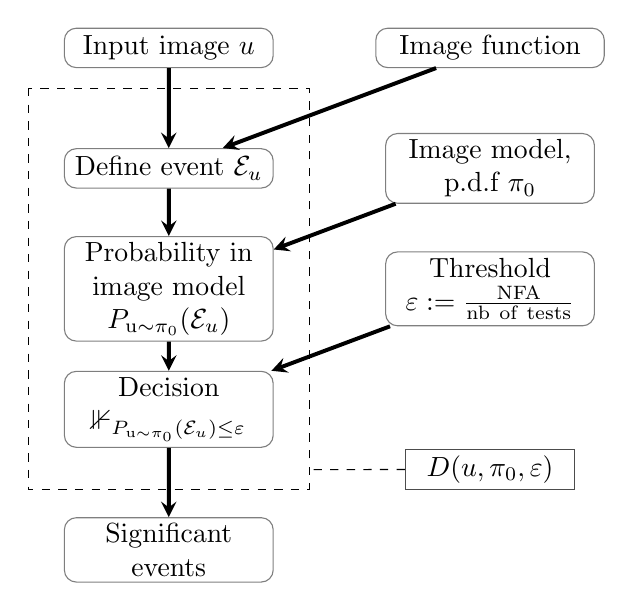
\begin{tikzpicture}[scale=1.02]
  \node[draw, minimum width = 1cm, minimum height = 0.5cm, text width=2.5cm, align=center, inner sep=0.5ex, rounded corners=1ex, fill=white, opacity=.5, text opacity = 1] (node 1) at (0.5,7) {Input image $u$};
  \node[draw, minimum width = 1cm, minimum height = 0.5cm, text width=2.5cm, align=center, inner sep=0.5ex, rounded corners=1ex, fill=white, opacity=.5, text opacity = 1] (node 2) at (0.5,5.5) {Define event $\mathcal{E}_u$};
  \node[draw, minimum width = 1cm, minimum height = 0.5cm, text width=2.5cm, align=center, inner sep=0.5ex, rounded corners=1ex, fill=white, opacity=.5, text opacity = 1] (node 3) at (0.5,4) {Probability in image model $P_{\bm{\mathrm{u}} \sim \pi_0}(\mathcal{E}_u)$};
  \node[draw, minimum width = 1cm, minimum height = 0.5cm, text width=2.5cm, align=center, inner sep=0.5ex, rounded corners=1ex, fill=white, opacity=.5, text opacity = 1] (node 4) at (0.5,2.5) {Decision $\mathbb{1}_{P_{\bm{\mathrm{u}} \sim \pi_0}(\mathcal{E}_u) \le \varepsilon}$};
  \node[draw, minimum width = 1cm, minimum height = 0.5cm, text width=2.5cm, align=center, inner sep=0.5ex, rounded corners=1ex, fill=white, opacity=.5, text opacity = 1] (node 5) at (0.5,0.75) {Significant events};
  

  \node[draw, minimum width = 1cm, minimum height = 0.5cm, text width=2.75cm, align=center, inner sep=0.5ex, rounded corners=1ex, fill=white, opacity=.5, text opacity = 1] (node 6) at (4.5,7) {Image function};
  \node[draw, minimum width = 1cm, minimum height = 0.5cm, text width=2.5cm, align=center, inner sep=0.5ex, rounded corners=1ex, fill=white, opacity=.5, text opacity = 1] (node 7) at (4.5,5.5) {Image model, p.d.f $\pi_0$};
  \node[draw, minimum width = 1cm, minimum height = 0.5cm, text width=2.5cm, align=center, inner sep=0.5ex, rounded corners=1ex, fill=white, opacity=.5, text opacity = 1] (node 8) at (4.5,4) {Threshold ${\varepsilon:= \frac{\operatorname{NFA}}{\text{nb of tests}}}$};

  
  \node[draw, minimum width = 1cm, minimum height = 0.5cm, text width=2cm, align=center, inner sep=0.5ex, fill=white, opacity=.7, text opacity = 1] (node 9) at (4.5,1.75) {$D(u,\pi_0,\varepsilon)$};  
  
  \draw [->, line width=.5mm,>=stealth, black] (node 1) -- (node 2);
  \draw [->, line width=.5mm,>=stealth, black] (node 2) -- (node 3);
  \draw [->, line width=.5mm,>=stealth, black] (node 3) -- (node 4);
  \draw [->, line width=.5mm,>=stealth, black] (node 4) -- (node 5);
  \draw [->, line width=.5mm,>=stealth, black] (node 6) -- (node 2);
  \draw [->, line width=.5mm,>=stealth, black] (node 7) -- (node 3);
  \draw [->, line width=.5mm,>=stealth, black] (node 8) -- (node 4);

  \draw[dashed] (-1.25,6.5) rectangle (2.25,1.5);

  \draw [dashed, black] (node 9) -- (2.25,1.75);
  
  % % general arrows
  % \node[draw, double arrow, shade, shading=axis, left color=white,right color=black,
  % minimum height=155mm, minimum width=5mm,
  % single arrow head extend=2mm,
  % anchor=west, rotate=0] at (-0.5,0) {};
  % \node[draw, single arrow, shade , shading=axis, bottom color=white,top color=black,
  % minimum height=145mm, minimum width=5mm,
  % single arrow head extend=2mm,
  % anchor=west, rotate=-90] at (-2,15) {};

  % % draw nodes
  % \node[draw, minimum width=4cm] (node 1) at (1,13) {sub-invariant measure};
  % \node[draw, minimum width=4cm] (node 2) at (1,10.75) {$\forall x \in X, \forall A \in \mathcal{B}, Q(x,A)=1$};              
  % \node[draw, minimum width=4cm] (node 3) at (1,9.25) {invariant measure};
  % \node[draw, minimum width=4cm] (node 4) at (1,7.75) {$\forall A \in \mathcal{B}, \underset{x \in X}{\sup}E_x(\tau_A) < +\infty$};
  % \node[draw, minimum width=4cm] (node 5) at (1,6.25) {invariant probability};
  % \node[draw, minimum width=4cm] (node 6) at (1,5) {strong aperiodicity};
  % \node[draw, minimum width=4cm] (node 7) at (1,3) {geometric recurrence};              
  % \node[draw, minimum width=3.2cm] (node 8) at (6.5,15) {Feller type condition};
  % \node[draw, minimum width=3.2cm] (node 9) at (6.5,13) {$\varphi$-irreducibility};    
  % \node[draw, minimum width=3.2cm] (node10) at (7,10) {Harris recurrence};
  % \node[draw, minimum width=3.2cm] (node11) at (7,7) {Harris positive recurrence};
  % \node[draw, minimum width=3.2cm] (node12) at (7,5) {Harris ergodicity};
  % \node[draw, minimum width=3.2cm] (node13) at (7,3) {geometric ergodicity};              
  % \node[draw, minimum width=3.2cm] (node14) at (12.5,15) {all compact sets are petite};              
  % \node[draw, minimum width=3.2cm] (node15) at (12.5,13) {$T$-chain};              
  % \node[draw, minimum width=3.2cm] (node16) at (12,10) {non-evanescence};
  % \node[draw, minimum width=3.2cm] (node17) at (12,7) {bounded probability};              
  % \node[draw] (node18) at (15,10) {DD1};
  % \node[draw] (node19) at (15,7) {DD2};
  % \node[draw] (node20) at (15,3) {DD3};
  % \node[draw] (node21) at (15,1) {DD4};

  % % intermediate node
  % \node[fill=black, minimum size=1pt] (node22) at (9.5,13) {};

  % % draw boxes
  % \draw[dashed] (4.5,10.5) rectangle (14,6.5);
  % \draw[dashed] (4.5,5.5) rectangle (14,2.5);

  % % draw logical arrows
  % \draw [->, line width=1mm,>=stealth, black] (node14) -- node[shape=circle, draw, inner sep=1pt, line width=1pt, right=3pt, fill=white] {4} (node15);
  % \draw [<->, line width=1mm, >=stealth, black] (node10) -- node[shape=circle, draw, inner sep=1pt, line width=1pt, below=3pt, fill=white] {5}(node16);
  % \draw [<->, line width=1mm, >=stealth, black] (node11) -- node[shape=circle, draw, inner sep=1pt, line width=1pt, below=3pt, fill=white] {5} (node17);    
  % \draw [->, line width=1mm, >=stealth, black] (node18) -- node[shape=circle, draw, inner sep=1pt, line width=1pt, below=3pt, fill=white] {6}(node16);
  % \draw [->, line width=1mm, >=stealth, black] (node19) -- node[shape=circle, draw, inner sep=1pt, line width=1pt, below=3pt, fill=white, fill = white] {7}(node17);
  % \draw [->, line width=1mm, >=stealth, black] (node20) -- node[shape=circle, draw, inner sep=1pt, line width=1pt, below=3pt, fill=white] {10}(node13);
  % \draw [->, line width=1mm, >=stealth, black] (node 7) -- node[shape=circle, draw, inner sep=1pt, line width=1pt, below=3pt, fill=white] {9} (node13);    
  % \draw [->, line width=1mm, >=stealth, black] (node21) -- (node20);
  % \draw [->, line width=1mm, >=stealth, black] (node11) -- node[shape=circle, draw, inner sep=1pt, line width=1pt, right=3pt, fill=white] {8} (node12);
  % \draw [->, line width=1mm, >=stealth, black] (node11) |- (node 5);
  % \draw [->, line width=1mm, >=stealth, black] (node 4) -| (node11);
  % \draw [->, line width=1mm, >=stealth, black] (node 2) -| (node10);
  % \draw [->, line width=1mm, >=stealth, black] (node10) |- node[shape=circle, draw, inner sep=1pt, line width=1pt, below=3pt, fill=white] {2} (node 3);
  % \draw [->, line width=1mm, >=stealth, black] (node 8) -- node[shape=circle, draw, inner sep=1pt, line width=1pt, below=3pt, fill=white] {3} (node14);
  % \draw [->, line width=1mm, >=stealth, black] (node 9) -- node[shape=circle, draw, inner sep=1pt, line width=1pt, below=3pt, fill=white] {1}(node 1);

  % % other nodes
  % \draw [-, black] (node 9) -- (node22);
  % \draw [-, black] (node15) -- (node22);
  % \draw [-, black] (node22) -- (9.5,10.5);
  % \draw [-, black] (node 6) -- (4.5,5);

  % % axis
  % \node at (1,-0.5) {\textbf{probability}};
  % \node at (13.5,-0.5) {\textbf{topology}};
  % \node[rotate = 90] at (-2.5,2) {\textbf{ergodicity}};
  % \node[rotate = 90] at (-2.5,14) {\textbf{stability}};    

\end{tikzpicture}
\end{flushleft}

%%% Local Variables:
%%% mode: latex
%%% TeX-master: "../../../../latex/report_thesis"
%%% End:
%%% Local Variables:
%%% mode: latex
%%% TeX-master: "main"
%%% End:

  \vspace{0.4cm}
  \textbf{Goal: } Find most similar patches in image (position maps) using \textit{a contrario} methods.}
  \headerbox{4. Patch similarity}{name=detection,column=2,span=1}{
  \begin{itemize}[leftmargin=*]
  \item $s$ similarity function between patches
  \item $\pi_0$ microtexture model, usually Gaussian \cite{galerne2011random}
  \item Two cases of \textbf{matching}:
    \begin{enumerate}
    \item \textbf{internal:} $\mathcal{E}_u := s(\bm{\mathrm{u}}, \bm{\mathrm{u}}) \le s(u,u)$ \newline
      (periodicity analysis)
    \item \textbf{template:} $\mathcal{E}_u := s(\bm{\mathrm{u}}, u_0) \le s(u,u_0)$ \newline
      (texture synthesis)
    \end{enumerate}
  \end{itemize}
%  \textbf{Question: } how to compute $\mathbb{1}_{P_{\bm{\mathrm{u}} \sim \pi_0}(\mathcal{E}_u) \le \varepsilon}$?
  \begin{center}
\begin{tikzpicture}
  \node[draw, minimum width = 1cm, minimum height = 0.5cm, text width=.95\linewidth, align=left, inner sep=0.5ex, rounded corners=1ex, fill=white, opacity=.9, text opacity = 1, blur shadow={shadow blur steps=5,shadow blur extra rounding=1.3pt}] (node 1) at (0,0) {\textbf{Proposition} \textit{(c.d.f and a contrario)} \newline We have \[\mathbb{1}_{P_{\bm{\mathrm{u}} \sim f}(\mathcal{E}_u) \le \varepsilon} = \mathbb{1}_{F(s(u,u)) \le \varepsilon} =  \mathbb{1}_{s(u,u) \le F^{-1}(\varepsilon)}\]
  \heart\textbf{\textcolor{blue}{Take-home 1:}} \textbf{A contrario similarity detection is simply thresholding with adaptive threshold.}};
\end{tikzpicture}
\end{center}
%%% Local Variables:
%%% mode: latex
%%% TeX-master: "main"
%%% End:

    \vspace{-0.3cm}
  \textbf{Question: } How to compute these c.d.f?
  \begin{enumerate}
  \item Focus on $\ell^2$ $\rightarrow$ Euclidean structure
  \item Depending on the similarity function, internal or template matching cases can be computed \textit{exactly}
  \end{enumerate}
  \posterthm{}{Internal matching and $\ell^2$}{
    Let $s(u,u)(x) = \| \mathbb{1}_{\omega}(u - \tau_x(u)) \|_2^2$ where ${\omega \subset \Omega}$ is a patch index.
    Suppose ${\veclet{u} \sim \mathcal{N}(0,C)}$ then
    \[ s(\veclet{u},\veclet{u})(x) \sim \summ{y \in \omega}{}{\lambda_y \xi_y}\]
    with $\lambda_y$ eigenvalues of $C_x = 2C - \tau_xC - \tau_{-x}C$ and $\xi_y$ independent $\chi_2$ r.v.}
  \vspace{0.08
    cm}
}

\headerbox{Conclusion}{name=conclusion, column=2, below=detection}{
  \begin{itemize}[leftmargin=*]
  \item Euclidean similarities allow for \textbf{fast computation} \vspace{-0.2cm}
  \item Thresholds for similarity detection are derived from \textbf{a contrario} methods \vspace{-0.2cm}
  \item Periodicity detection algorithm, links with \textbf{co-occurence} matrix methods \cite{conners1980toward} 
  \end{itemize}
%  \vspace{-0.1cm}
}

\headerbox{Bibliography}{name=biblio, column=2, below=conclusion}{
\printbibliography[heading=none]
}
% ----------------------------------------------------------------------------------------
%	OTHER INSTRUMENTATION
%----------------------------------------------------------------------------------------
\headerbox{2. Comparing patches}{name=comparing,span=1,column=0, below=introduction}{
  \small
  %To reduce this block to 1 column width, remove 'span=2'

% \begin{center}
% \resizebox{0.9\textwidth}{!}{\begin{minipage}{\textwidth}
% \begin{tabular}{l l l l}
% \toprule
% \textbf{Name} & \textbf{Manufacturer} & \textbf{Receivers} & \textbf{Availability}\\
% \midrule
% MTA (requires two synchronized) & HP & Sampler & Discontinued \\
% LSNA & Agilent & Sampler & Discontinued \\
% PNA-X + Nonlinear option & Agilent & Mixer & \$\$ \\
%   ZVA + Nonlinear option & Rohde and Schwarz & Mixer &  \$\$ \\
%   ZVA + Nonlinear option & Rohde and Schwarz & Mixer &  \$\$ \\
%   ZVA + Nonlinear option & Rohde and Schwarz & Mixer &  \$\$ \\
%   ZVA + Nonlinear option & Rohde and Schwarz & Mixer &  \$\$ \\
%   ZVA + Nonlinear option & Rohde and Schwarz & Mixer &  \$\$ \\
%   ZVA + Nonlinear option & Rohde and Schwarz & Mixer &  \$\$ \\
%   ZVA + Nonlinear option & Rohde and Schwarz & Mixer &  \$\$ \\
%   ZVA + Nonlinear option & Rohde and Schwarz & Mixer &  \$\$ \\
%   ZVA + Nonlinear option & Rohde and Schwarz & Mixer &  \$\$ \\
%   ZVA + Nonlinear option & Rohde and Schwarz & Mixer &  \$\$ \\
%   ZVA + Nonlinear option & Rohde and Schwarz & Mixer &  \$\$ \\
%   ZVA + Nonlinear option & Rohde and Schwarz & Mixer &  \$\$ \\
% SWAP X-402 & VTD & Sampler & Discontinued \\
% \bottomrule
% \end{tabular}
% \end{minipage}}
% \end{center}
  Let $u$ be an image defined over $\Omega \subset \Z^2$. \newline
  To compare patches in images several comparison functions are available \cite{deledalle2012compare}:
  \vspace{-0.2cm}
  \begin{itemize}[leftmargin=*]
  \item $\ell^p$ norms (especially \textcolor{red_mat}{$\ell^1$}, \textcolor{blue_mat}{$\ell^2$} and \textcolor{green_mat}{$\ell^{\infty}$})
  \item Directional measurements (Euclidean scalar product, angle measurements)
  \end{itemize}
  \vspace{-0.5cm}
%   \textbf{Observation: } trade-off between \textit{rigidity} and \textit{innovation}.
%   \begin{center}
%   %\begin{left}
%     \begin{tikzpicture}[scale=0.7]
      \node[inner sep=0pt] (input) at (0,0)
      {\includegraphics[width=.2\textwidth]{./figures/export_fig_out.png}};
      \node[] (4) at (-2.4,-0.6) {\tiny $4$};
      \node[] (8) at (-2.4,0.6) {\tiny $8$};
      \node[] (exp) at (-2.5,2) {\tiny $\times 10^{-3}$};      
      \node[] (02) at (-.5,-2) {\tiny $0.2$};
      \node[] (03) at (.5,-2) {\tiny $0.3$};            
      \node[inner sep=0pt] (input) at (-1.25,-2.25)
      {\includegraphics[width=.06\textwidth]{./figures/orig_skew.png}};
      \node[inner sep=0pt] (input) at (2,-2.25)
      {\includegraphics[width=.06\textwidth]{./figures/noisy_skew.png}};
      \draw [->, red, line width=0.5mm, >=stealth] (-1,-2.25) --node[below=1mm, black] {\tiny noise std} (1.2,-2.25);
      \draw [->, red, line width=0.5mm, >=stealth] (-2.6,-1.75) -- (-2.6,1.75);
      \node[left=3mm, black, text width = 3cm, rotate=90] at (-2.5,2.5) {\tiny \% of pixels detected};
\end{tikzpicture}      
%%% Local Variables:
%%% mode: latex
%%% TeX-master: "main"
%%% End:

%   % \end{left}
% \hspace{10pt}
% \begin{tikzpicture}
%   \node[] at (0,0) {};
%       \draw [<->,line width = 1mm, >=stealth] (-1.5,3) to [out=20,in=160]node[below = 1mm, text width = 2.7cm]{\begin{center}  \small real world images + geometric experiments to illustrate this rigidity/innovation trade-off \end{center}} (1.5,3) [];
%     \end{tikzpicture}
% \hspace{10pt}
     \begin{center}
       \begin{tikzpicture}[scale=1.1]
      \node[inner sep=0pt] (input) at (0,2)
      {\includegraphics[width=.25\textwidth]{/home/debortoli/research/patch_sim/res_percep/contrast_00_L2_20_superp.png}};
      \node[] at (0,1) {\scriptsize \textcolor{blue_mat}{$\ell^2$}};
      \node[inner sep=0pt] (input) at (2,2)
      {\includegraphics[width=.25\textwidth]{/home/debortoli/research/patch_sim/res_percep/contrast_00_L1_20_superp.png}};
      \node[] at (2,1) {\scriptsize \textcolor{red_mat}{$\ell^1$}};

      \node[inner sep=0pt] (input) at (4,2)
     {\includegraphics[width=.25\textwidth]{/home/debortoli/research/patch_sim/res_percep/contrast_00_Linfinite_20_superp.png}};
      \node[] at (4,1) {\scriptsize \textcolor{green_mat}{$\ell^{\infty}$}};

      \node[inner sep=0pt] (input) at (0,0)
      {\includegraphics[width=.25\textwidth]{/home/debortoli/research/patch_sim/res_percep/contrast_00_ps_20_superp.png}};
      \node[] at (0,-1) {\scriptsize Scalar product};

      \node[inner sep=0pt] (input) at (2,0)
      {\includegraphics[width=.25\textwidth]{/home/debortoli/research/patch_sim/res_percep/contrast_00_cos_20_superp.png}};
      \node[] at (2,-1) {\scriptsize Cosine};

      \node[text width = 1.75cm, inner sep = 0pt] at (4,0) {\begin{center}\footnotesize \textbf{20} best matches for top-left patch.\end{center}};
\end{tikzpicture}      

%%% Local Variables:
%%% mode: latex
%%% TeX-master: "main"
%%% End:

       \end{center}
%   \end{center}
% \begin{figure}
%   \subfloat{\includegraphics[width=.18\linewidth]{contrast_00_L2_20_superp.png}} \hfill
%   \subfloat{\includegraphics[width=.18\linewidth]{contrast_00_L1_20_superp.png}} \hfill
%   \subfloat{\includegraphics[width=.18\linewidth]{contrast_00_Linfinite_20_superp.png}} \hfill
%   \subfloat{\includegraphics[width=.18\linewidth]{contrast_00_ps_20_superp.png}} \hfill
%   \subfloat{\includegraphics[width=.18\linewidth]{contrast_00_cos_20_superp.png}} \hfill \\
% \end{figure}
}


%----------------------------------------------------------------------------------------
%	MIXER vs. SAMPLERS
%----------------------------------------------------------------------------------------
% \headerbox{Receiver: Mixer vs. Sampler}{name=comparing,span=2,column=1,row=1, below=instruments}{
% \begin{center}
% \includegraphics[width=1\linewidth]{RECEIVER.pdf}
% \end{center}
% }


%----------------------------------------------------------------------------------------
%	MEASUREMENT SETUP
%----------------------------------------------------------------------------------------
\headerbox{5. Periodicity analysis}{name=periodicity,span=2,column=0,below=comparing}{
  \small
  \textbf{Goal: } Given $u$ with a periodic pattern $P$ find the underlying lattice $\mathcal{L} = (e_1,e_2)$. Let $X$ be a set of vertices.
  \posterassumption{}{Deformed lattice hypothesis}{
    \[ \forall x \in X, \forall y \in \mathcal{N}_x, \exists (m_{\lbrace x,y \rbrace}, n_{\lbrace x, y \rbrace}) \in \Z^2, x - y = m_{\lbrace x,y \rbrace} e_1 + n_{\lbrace x,y \rbrace} e_2 + \sigma Z_{\lbrace x,y \rbrace} \]
    where $\mathcal{N}_x$ is a neighborhood of $x$ and $Z_{\lbrace x,y \rbrace}$ are independent standard Gaussian r.v.}
  \heart\textbf{\textcolor{blue}{Take-home 2:}} \textbf{This hypothesis is naturally translated in a graphical model and reduces to parameters estimation of $(e_1,e_2,m_{\lbrace x,y \rbrace},n_{\lbrace x,y \rbrace},\sigma)$.}
  \vspace{-0.3cm}
  \[ \underbrace{L(X)}_{\text{log-likelihood}} := -C\log(\sigma^2) - \frac{1}{2\sigma^2}\underbrace{\left( \summ{x \in X, y \in \mathcal{N}_x}{}{\| (m_{\lbrace x,y \rbrace}e_1+n_{\lbrace x,y \rbrace}e_2) - (x-y) \|^2} + \overbrace{r(m_{\lbrace x,y \rbrace}, n_{\lbrace x, y \rbrace},e_1,e_2,\delta,\eta)}^{\text{regularization}} \right)}_{E_{\delta,\eta}(m_{\lbrace x,y \rbrace}, n_{\lbrace x, y \rbrace},e_1,e_2)}\]
  \vspace{-0.5cm}
  \begin{algorithm}[H]
    \small
\caption{Lattice detection -- $L(\delta,\eta,N)$}
\begin{algorithmic}
\REQUIRE{$\delta$, $\eta$ and $N$ set by user}
% \REQUIRE{$\delta \eta \ge 3 \|Z\|$}
% \STATE $(e_1^0,e_1^0)$ randomly chosen in the unit sphere
\FOR{$n=0$ to $N-1$}
\STATE $(\tilde{m}_{\lbrace x,y \rbrace},\tilde{n}_{\lbrace x,y \rbrace}) \ \leftarrow \underset{\mathbb{R}^2}{\operatorname{argmin}} \ E_{\delta,0}(m_{\lbrace x,y \rbrace},n_{\lbrace x,y \rbrace},e_1^n,e_2^n)$
\STATE $(m_{\lbrace x,y \rbrace}^{n+1}, n_{\lbrace x,y \rbrace}^{n+1}) \ \leftarrow \ \operatorname{argmin} \ (E_{\delta,0}(\operatorname{round}\left((\tilde{m}_{\lbrace x,y \rbrace}, \tilde{n}_{\lbrace x,y \rbrace})\right),e_1^n,e_2^n), E_{\delta,0}(m_{\lbrace x,y \rbrace}^n,n_{\lbrace x,y \rbrace}^n,e_1^n,e_2^n))$
\STATE $(e_1^{n+1},e_2^{n+1}) \ \leftarrow \ \underset{\left(\mathbb{R}^2\right)^2}{\operatorname{argmin}} \ E_{0,\eta}(m_{\lbrace x,y \rbrace}^{n+1}, n_{\lbrace x,y \rbrace}^{n+1}, e_1,e_2)$
\ENDFOR
% \STATE compute $\sigma^{N}$, compute $L^N$
% \RETURN $(m_{\lbrace x,y \rbrace}^N, n_{\lbrace x,y \rbrace}^N,e_1^N,e_2^N,\sigma^N,L^N)$
\end{algorithmic}
\end{algorithm}
\vspace{-1cm}
\begin{center}
  \begin{tikzpicture}
  \node[inner sep=0pt] (input) at (0,0)
  {\includegraphics[width=.2\textwidth]{./figures/Iout.png}};
  \node[inner sep=0pt] (a_contrario) at (6,0)
    {\includegraphics[width=.2\textwidth]{./figures/d_true_out.png}};
  \node[inner sep=0pt] (vertice) at (12.65,0.65)
    {\includegraphics[width=.2\textwidth]{./figures/vertice_im.png}};
  \node[inner sep=0pt] (periodicity) at (12,0)
  {\includegraphics[width=.2\textwidth]{./figures/super.png}};
  \draw [->, line width=.5mm,>=stealth, black] (input) -- node[above=3pt]{$D(u, \pi_0,\varepsilon)$} (a_contrario);
  \draw [->, line width=.5mm,>=stealth, black] (a_contrario) -- node[above=3pt]{$L(\delta,\eta,N)$}(periodicity);
\end{tikzpicture}
%%% Local Variables:
%%% mode: latex
%%% TeX-master: "main"
%%% End:

\end{center}
\begin{center}

  \begin{tikzpicture}[scale=1]
      \node[inner sep=0pt] (input1) at (0,0)
      {\includegraphics[width=.139\textwidth]{/home/debortoli/img/simoncelli/simoncelli_original/img_05.png}};
      \node[inner sep=0pt] (output2) at (4.2,0.5)
      {\includegraphics[width=.139\textwidth]{./vertice_im5.png}};                  
      \node[inner sep=0pt] (output1) at (3.7,0)
      {\includegraphics[width=.139\textwidth]{./super_5.png}};
      \draw [->,red,line width = .5mm, >=stealth] (input1.north) to [out=35,in=145]node[below = 2.5mm, black]{$\text{duration} = 7.8s$} (output1.north);
      \node[inner sep=0pt] (input2) at (8.3,0)
      {\includegraphics[width=.139\textwidth]{/home/debortoli/img/simoncelli/simoncelli_original/img_06.png}};
      \node[inner sep=0pt] (output2) at (12.5,0.5)
      {\includegraphics[width=.139\textwidth]{./vertice_im6.png}};      
      \node[inner sep=0pt] (output2) at (12,0)
      {\includegraphics[width=.139\textwidth]{./super_6.png}};
      \draw [->,red,line width = .5mm, >=stealth] (input2.north) to  [out=35,in=145]node[below = 2.5mm, black]{$\text{duration} = 8.6s$} (output2.north);      
\end{tikzpicture}      

%%% Local Variables:
%%% mode: latex
%%% TeX-master: "main"
%%% End:

  \end{center}
  \posterprop{}{Finite time convergence}{
    Under conditions on $(\delta,\eta)$ Algorithm $1$ converges in \textbf{finite time}.
    Moreover the log-likelihood is increased at each step.
  }
  \vspace{-0.3cm}
  \textbf{Problems \& remarks: }
  \vspace{-0.2cm}
\begin{itemize}[leftmargin=*]
\item Conditions not satisfied in practice, \textbf{but} finite time convergence still observed
  \vspace{-0.2cm}
\item Can be written as \textbf{EM} algorithm
\end{itemize}
% The setup includes \textbf{two LSNAs simultaneously}. One is dedicated to RF (sampler based downconversion), the other one samples directly the LF stimulus. The purpose is to investigate \textbf{low-frequencies $S_{22}$} of the DUT under RF large signal conditions.
% \begin{center}
% \includegraphics[width=\linewidth]{BENCH.pdf}
% \small \textit{Low-frequency measurement of drain supply envelope-bandwidth impedance for supply-modulated PAs}
% \end{center}
}


%----------------------------------------------------------------------------------------
%	CONCLUSION
%----------------------------------------------------------------------------------------
%\headerbox{Conclusion}{name=conclusion,column=1,below=periodicity,span=2}{
% This new project will enable a new RF measurement capability by enabling an instrument that currently does not exist on the market. Some additional benefits include:
% \vspace{-0.2cm}
% \begin{itemize} 
% \item frequency range extension of NI RF instrument products currently available;
% \vspace{-0.2cm}
% \item sampler architecture offers a unique multi-scale time analysis possibility (e.g. signal and carrier domains);
% \vspace{-0.2cm}
% \item can be implemented with various ADCs and downconverters (e.g. THAs);
% \vspace{-0.2cm}
% \item 100\% LabVIEW environment;
% \vspace{-0.2cm}
% \item goal is to offer open-source LabVIEW software for user measurement flexibility.
% \end{itemize}
%}


%----------------------------------------------------------------------------------------
%	REFERENCES
%----------------------------------------------------------------------------------------

%\headerbox{References}{name=references,column=2,below=periodicity}{

%\smaller % Reduce the font size in this block
%\renewcommand{\section}[2]{\vskip 0.05em} % Get rid of the default "References" section title
%\nocite{*} % Insert publications even if they are not cited in the poster

%\bibliographystyle{unsrt}
%\bibliographystyle{IEEEtran}
%\bibliography{biblio} % Use biblio.bib as the bibliography file
%}


%----------------------------------------------------------------------------------------
%	ACKNOWLEDGEMENTS
%----------------------------------------------------------------------------------------

% \headerbox{Acknowledgements}{name=acknowledgements,column=0,below=conclusion, above=bottom,span=3}{
% \smaller 
% This work is funded by National Instruments (Dr. Truchard) through a charitable donation. We would like to acknowledge DARPA (Dr. Greene) and ONR (Dr. Maki) for funding the initial part of this work under grant N00014-11-1-0931. \hfill \tiny \textit{Poster downloaded from} \textbf{www.microwave.fr}
% } 


\end{poster}

\end{document}
%%% Local Variables:
%%% mode: latex
%%% TeX-master: t
%%% End:
